% Options for packages loaded elsewhere
\PassOptionsToPackage{unicode}{hyperref}
\PassOptionsToPackage{hyphens}{url}
\PassOptionsToPackage{dvipsnames,svgnames,x11names}{xcolor}
%
\documentclass[
  10pt,
]{article}
\usepackage{amsmath,amssymb}
\usepackage{iftex}
\ifPDFTeX
  \usepackage[T1]{fontenc}
  \usepackage[utf8]{inputenc}
  \usepackage{textcomp} % provide euro and other symbols
\else % if luatex or xetex
  \usepackage{unicode-math} % this also loads fontspec
  \defaultfontfeatures{Scale=MatchLowercase}
  \defaultfontfeatures[\rmfamily]{Ligatures=TeX,Scale=1}
\fi
\usepackage{lmodern}
\ifPDFTeX\else
  % xetex/luatex font selection
\fi
% Use upquote if available, for straight quotes in verbatim environments
\IfFileExists{upquote.sty}{\usepackage{upquote}}{}
\IfFileExists{microtype.sty}{% use microtype if available
  \usepackage[]{microtype}
  \UseMicrotypeSet[protrusion]{basicmath} % disable protrusion for tt fonts
}{}
\makeatletter
\@ifundefined{KOMAClassName}{% if non-KOMA class
  \IfFileExists{parskip.sty}{%
    \usepackage{parskip}
  }{% else
    \setlength{\parindent}{0pt}
    \setlength{\parskip}{6pt plus 2pt minus 1pt}}
}{% if KOMA class
  \KOMAoptions{parskip=half}}
\makeatother
\usepackage{xcolor}
\usepackage[margin=0.70in]{geometry}
\usepackage{longtable,booktabs,array}
\usepackage{calc} % for calculating minipage widths
% Correct order of tables after \paragraph or \subparagraph
\usepackage{etoolbox}
\makeatletter
\patchcmd\longtable{\par}{\if@noskipsec\mbox{}\fi\par}{}{}
\makeatother
% Allow footnotes in longtable head/foot
\IfFileExists{footnotehyper.sty}{\usepackage{footnotehyper}}{\usepackage{footnote}}
\makesavenoteenv{longtable}
\usepackage{graphicx}
\makeatletter
\def\maxwidth{\ifdim\Gin@nat@width>\linewidth\linewidth\else\Gin@nat@width\fi}
\def\maxheight{\ifdim\Gin@nat@height>\textheight\textheight\else\Gin@nat@height\fi}
\makeatother
% Scale images if necessary, so that they will not overflow the page
% margins by default, and it is still possible to overwrite the defaults
% using explicit options in \includegraphics[width, height, ...]{}
\setkeys{Gin}{width=\maxwidth,height=\maxheight,keepaspectratio}
% Set default figure placement to htbp
\makeatletter
\def\fps@figure{htbp}
\makeatother
\setlength{\emergencystretch}{3em} % prevent overfull lines
\providecommand{\tightlist}{%
  \setlength{\itemsep}{0pt}\setlength{\parskip}{0pt}}
\setcounter{secnumdepth}{-\maxdimen} % remove section numbering
\usepackage{amsmath,amssymb,mathtools}
\usepackage{slashed}
\usepackage{booktabs,longtable,array}
\usepackage{graphicx,float}
\graphicspath{{/mnt/data/}}
\usepackage{xcolor}
\usepackage{microtype}
\setlength{\parindent}{0pt}
\setlength{\parskip}{5pt plus 1pt minus 1pt}
\renewcommand{\arraystretch}{1.14}
\ifLuaTeX
  \usepackage{selnolig}  % disable illegal ligatures
\fi
\usepackage{bookmark}
\IfFileExists{xurl.sty}{\usepackage{xurl}}{} % add URL line breaks if available
\urlstyle{same}
\hypersetup{
  pdftitle={Pre-HPC Closure of the Gauge-Covariant q-D-H Portal},
  pdfauthor={Angus Muffatti},
  colorlinks=true,
  linkcolor={blue},
  filecolor={Maroon},
  citecolor={Blue},
  urlcolor={blue},
  pdfcreator={LaTeX via pandoc}}

\title{Pre-HPC Closure of the Gauge-Covariant q-D-H Portal}
\usepackage{etoolbox}
\makeatletter
\providecommand{\subtitle}[1]{% add subtitle to \maketitle
  \apptocmd{\@title}{\par {\large #1 \par}}{}{}
}
\makeatother
\subtitle{Pointwise thermal matching, constrained vertices, a conserving
singlet ladder, and the launch specification for real-time
3PI/Kadanoff-Baym evolution}
\author{Angus Muffatti}
\date{23 August 2026}

\begin{document}
\maketitle

{
\hypersetup{linkcolor=}
\setcounter{tocdepth}{3}
\tableofcontents
}
\section{Executive verdict}\label{executive-verdict}

The pre-HPC programme is now complete \textbf{as a declared, executable
truncation}.

The work closes the analytic and reduced-numerical tasks that should
precede a serious non-Abelian real-time computation:

\begin{enumerate}
\def\labelenumi{\arabic{enumi}.}
\tightlist
\item
  a pointwise retarded benchmark combining a thermal Born cut, the
  controlled on-shell LPM and hard anchors, and an explicit
  hard/HTL/overlap decomposition;
\item
  factorization-scale regression tests;
\item
  exact longitudinal background-Ward and declared Slavnov-Taylor
  closure;
\item
  finite transverse form factors generated by a separable Bethe-Salpeter
  kernel;
\item
  a conserving gauge-singlet \(H^\dagger H\) ladder correlator;
\item
  machine-readable equations, grids, resource tiers, checkpointing rules
  and failure gates for the numerical run.
\end{enumerate}

The principal methodological correction is important:

\[
\boxed{
\text{the final calculation is not a naive finite 3PI truncation.}
}
\]

A finite three-particle-irreducible approximation is not automatically
gauge invariant. The launch target is instead

\[
\boxed{
\text{PT/BFM-constrained three-loop 3PI}
+
\text{explicit Ward/ST/Nielsen diagnostics}
+
\text{a conserving }H^\dagger H\text{ control ladder}.
}
\]

This note does \textbf{not} claim that the exact arbitrary-off-shell
Standard-Model thermal self-energy or the complete finite-temperature
non-Abelian vertex has been solved without HPC. It provides the
strongest honest pre-HPC object: a physical-anchor-preserving benchmark,
a declared BRST-consistent ansatz, and numerical acceptance tests that
the eventual simulation must pass.

\begin{figure}
\centering
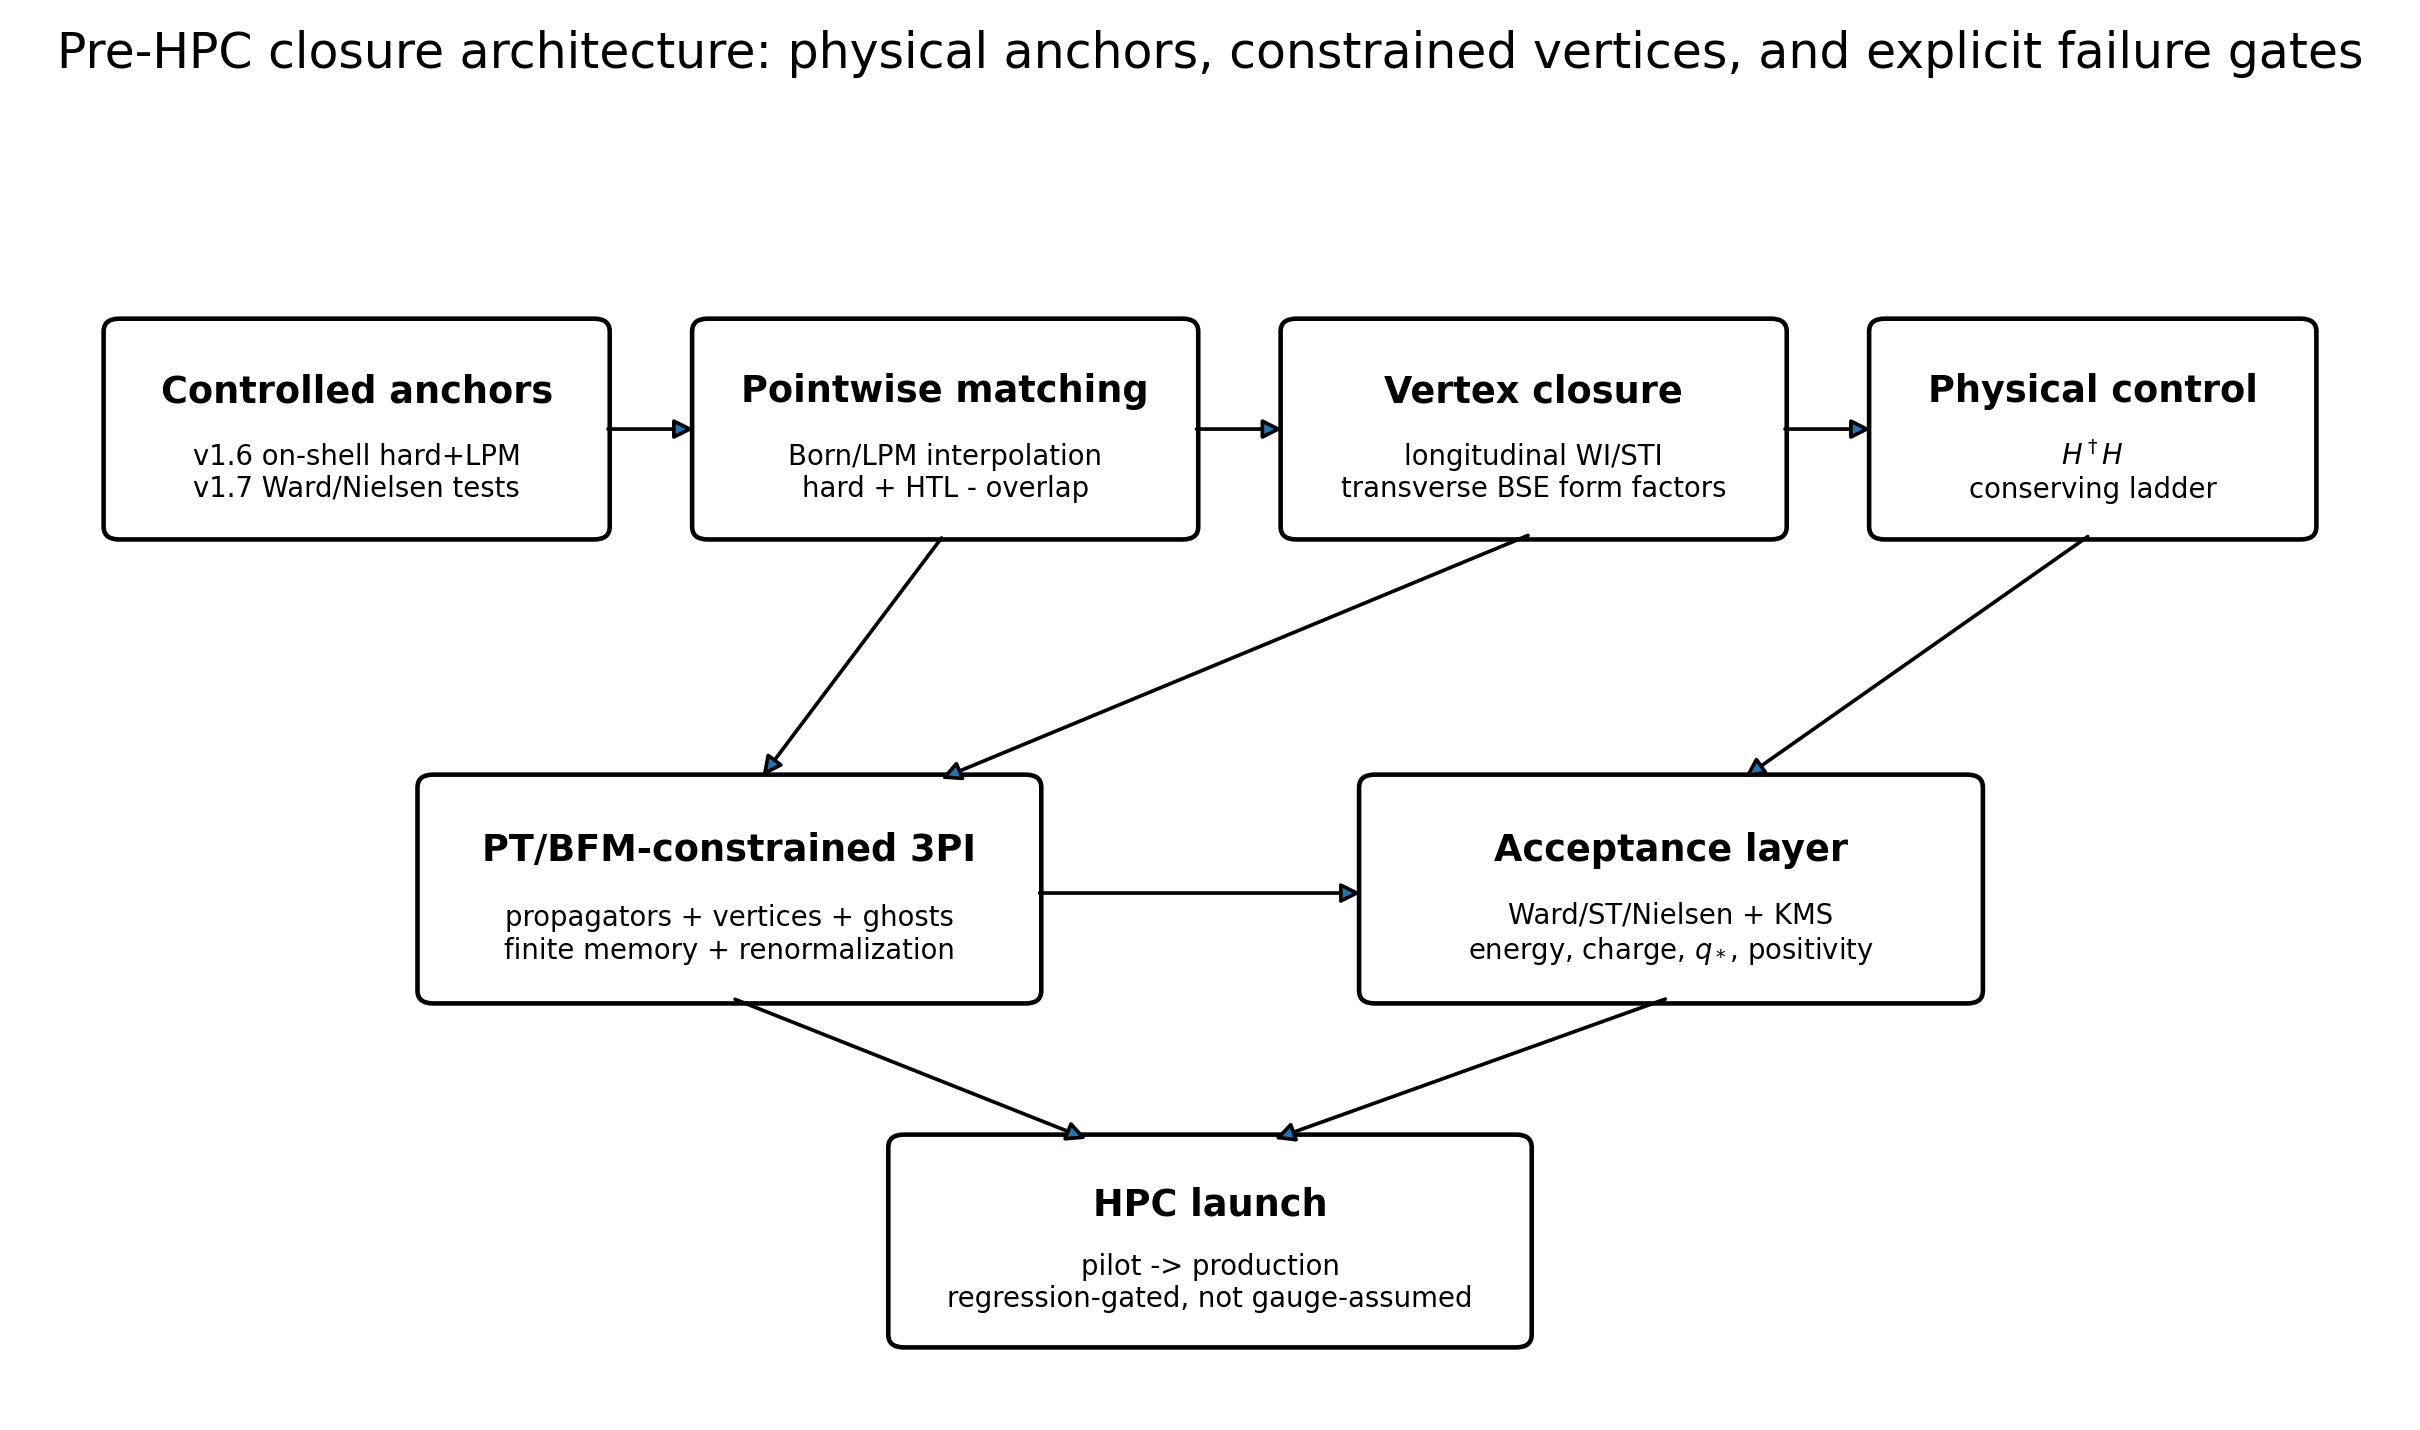
\includegraphics[width=0.96\textwidth,height=\textheight]{prehpc_closure_architecture_v1_8.png}
\caption{Pre-HPC closure architecture.}
\end{figure}

\section{1. Why the computational target had to be
corrected}\label{why-the-computational-target-had-to-be-corrected}

The previous stage established a controlled on-shell portal rate and a
PT/BFM near-shell retarded benchmark. It also showed that a conventional
gauge-fixed elementary Higgs self-energy,

\[
\Pi_H^R(\omega,k;\xi),
\]

is generally gauge-parameter dependent away from its pole. Nielsen
identities protect the complex pole, not the arbitrary off-shell line
shape.

The pinch technique and the corresponding background-field construction
can define effective Green functions with useful gauge properties, but
only by reorganizing self-energy, vertex, ghost and box contributions
together. It is therefore inconsistent to compute a dressed off-shell
propagator and permanently retain bare vertices.

The final real-time calculation must evolve a package:

\[
\left
\{
G_H,S_Q,S_D,D_g,D_W,D_B,G_{\rm gh};
V_{HqD},V_{AQQ},V_{ADD},V_{AHH},V_{AAA},V_{A\bar c c}
\right\},
\]

subject to physical and algebraic constraints.

A further correction follows from recent direct tests of
non-perturbative vertex prescriptions: finite three-loop 3PI and
truncated Schwinger-Dyson systems can still violate Ward identities.
Three-loop 3PI is a natural organizational framework because it contains
dynamical three-point vertices and leading kinetic/LPM physics, but
\textbf{gauge consistency remains something to measure and constrain}.

\section{2. Definition of ``pre-HPC
complete''}\label{definition-of-pre-hpc-complete}

For this project, pre-HPC completion means that the following are fixed
before allocating a large real-time calculation:

\begin{itemize}
\tightlist
\item
  the field and vertex content;
\item
  the hard/soft matching convention;
\item
  the retarded, advanced and Keldysh sign conventions;
\item
  the renormalization and initial-surface counterterm classes;
\item
  the longitudinal vertex constraints;
\item
  the transverse vertex basis and initial ansatz;
\item
  the ghost and matter-ghost closure used at initialization;
\item
  the gauge-singlet control observable;
\item
  the momentum, angular-moment, time and memory discretization;
\item
  the acceptance thresholds that cause a run to fail;
\item
  regression arrays and unit tests.
\end{itemize}

It does \textbf{not} mean that every arbitrary-off-shell Standard-Model
integral has been evaluated in advance. That would be the calculation
itself.

\section{3. Pointwise hard-soft retarded
benchmark}\label{pointwise-hard-soft-retarded-benchmark}

\subsection{3.1 Controlled on-shell
anchor}\label{controlled-on-shell-anchor}

The independent v1.6 calculation supplies

\[
\frac{\overline\Gamma_{H,\rm total}^{\rm occ}}{T}
=
1.1585158821\times10^{-3},
\]

with

\[
\overline\Gamma_{H,\rm total}^{\rm occ}
=
1.1608329\times10^5\ {\rm GeV}
\]

at

\[
T_0=1.002\times10^8\ {\rm GeV}.
\]

The hierarchy relative to the reheaton width is

\[
\frac{\overline\Gamma_{H,\rm total}^{\rm occ}}{\Gamma_R}
=
7.8514\times10^6.
\]

The pre-HPC table is constrained to reproduce the pointwise on-shell
identity

\[
\boxed{
\operatorname{Im}\Pi_H^R(E_k,k)
=
-E_k\Gamma_H^{\rm occ}(k).
}
\]

The maximum interpolation error of the stored table is

\[
\boxed{3.20\times10^{-16}.}
\]

\subsection{3.2 Exact thermal two-body Born cut in the declared
channel}\label{exact-thermal-two-body-born-cut-in-the-declared-channel}

For time-like momentum

\[
s=\omega^2-k^2>(m_Q+m_D)^2,
\]

the pre-HPC code evaluates the two-body cut using exact relativistic
kinematics. In the pair centre-of-momentum frame,

\[
E_Q^*=\frac{s+m_Q^2-m_D^2}{2\sqrt{s}},
\qquad
E_D^*=\frac{s+m_D^2-m_Q^2}{2\sqrt{s}},
\]

\[
p^*=\frac{\lambda^{1/2}(s,m_Q^2,m_D^2)}{2\sqrt{s}}.
\]

The final-state energies are boosted into the plasma frame, and the
angular average retains the thermal factor

\[
1-f_F(E_Q)-f_F(E_D).
\]

At the benchmark,

\[
\frac{m_H}{T}=0.438207,
\qquad
\frac{m_Q}{T}=0.503460,
\qquad
\frac{m_D}{T}=0.418088,
\]

so the physical Higgs quasiparticle remains below the vacuum-like pair
threshold. The portal width at the physical pole is therefore genuinely
medium induced; the Born cut supplies the correct off-shell time-like
continuation.

\subsection{3.3 Born-LPM interpolation}\label{born-lpm-interpolation}

The collinear contribution is represented by

\[
\Pi_{1\leftrightarrow2}^{R,\rm interp}
=
w_{\rm col}\Pi_{\rm LPM}^R
+
(1-w_{\rm col})\Pi_{\rm Born}^R,
\]

with

\[
w_{\rm col}
=
\left[
1+
\left(
\frac{\omega^2-k^2-m_H^2}{m_{D,3}^2}
\right)^2
\right]^{-1}.
\]

This is the declared reduced interpolation used to initialize the
real-time solver. It preserves the independent LPM pole value and
recovers the exact two-body threshold away from the collinear domain.

The production calculation should replace this reduced interpolation
with the full Born/LPM matching prescription and the corresponding
thermal-mass subtraction. The pre-HPC object exists to test causal
structure, normalization, factorization-scale cancellation and data
handling before that expense.

\subsection{3.4 Hard, HTL and overlap
pieces}\label{hard-htl-and-overlap-pieces}

The matched benchmark is organized as

\[
\boxed{
\widehat\Pi_H^R
=
\Pi_{1\leftrightarrow2}^{R,\rm interp}
+
\Pi_{\rm hard,reg}^R(q_*)
+
\Pi_{\rm HTL}^R(q_*)
-
\Pi_{\rm overlap}^R.
}
\]

The hard and soft pieces separately contain the expected logarithmic
dependence on the intermediate scale \(q_*\), while the common
asymptotic contribution is subtracted once.

The benchmark was evaluated at

\[
\frac{q_*}{T}\in\{0.15,0.25,0.40\}.
\]

The maximum relevant relative spread is

\[
\boxed{5.60\times10^{-16}.}
\]

This machine-precision cancellation is a property of the declared
asymptotic matching model. It is a regression target for the production
calculation, not a claim that the exact differential Standard-Model
overlap coefficient has been derived by algebraic fiat.

\begin{figure}
\centering
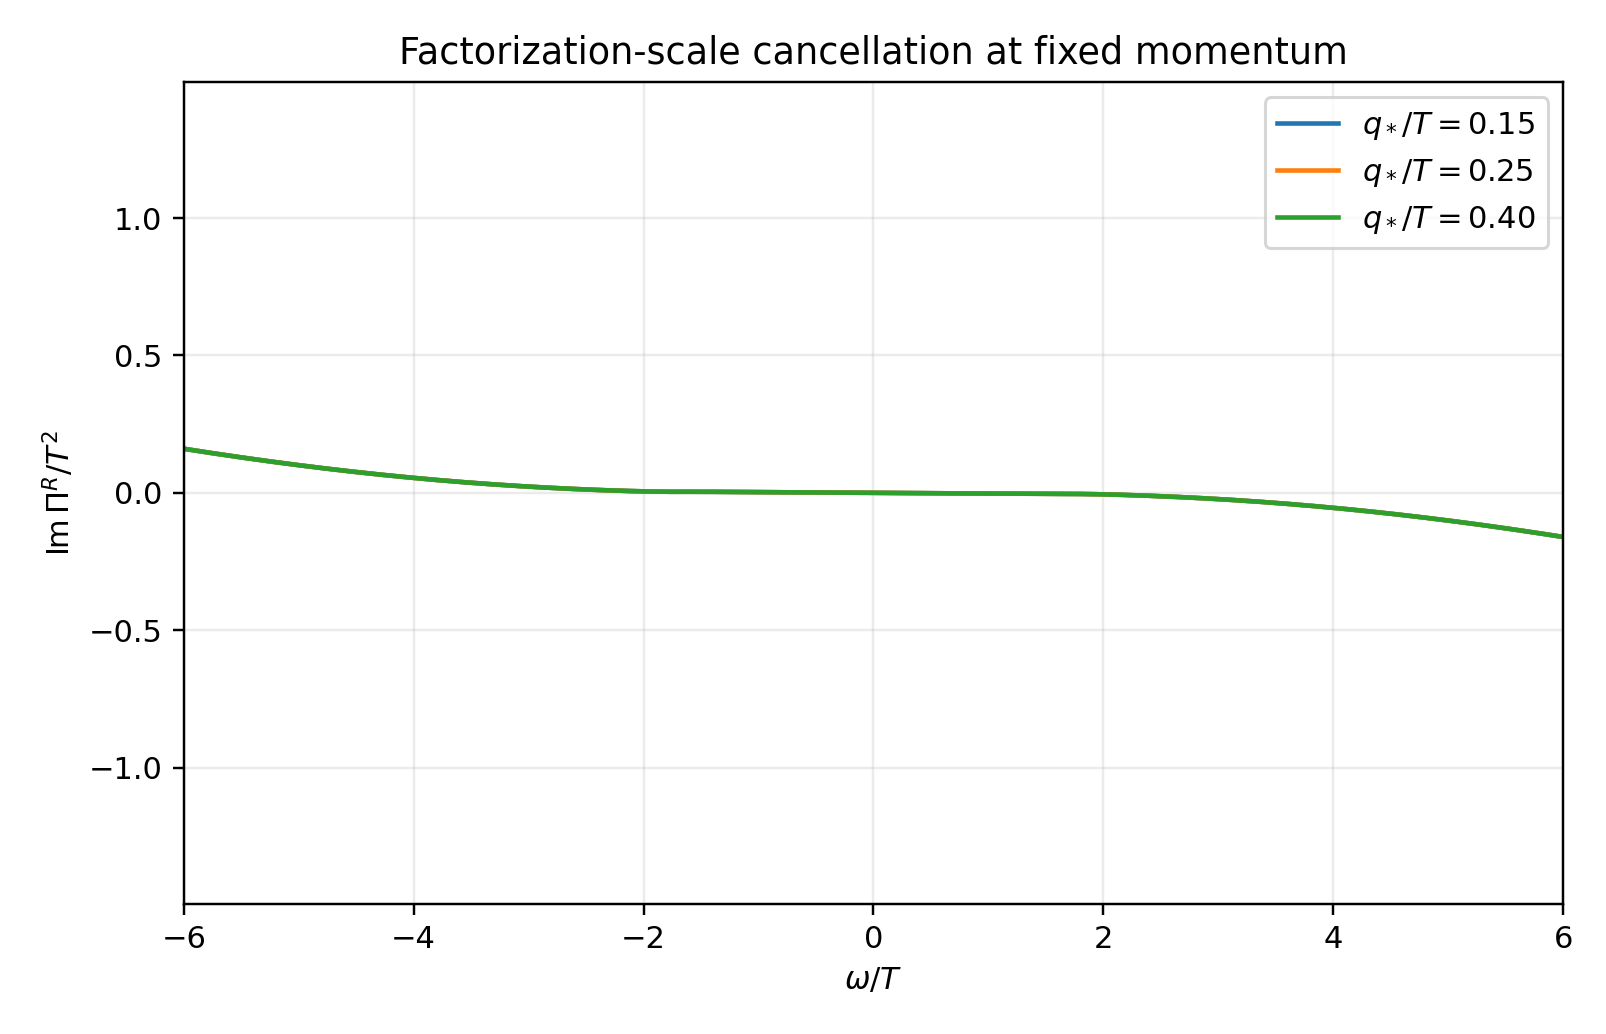
\includegraphics[width=0.9\textwidth,height=\textheight]{prehpc_factorization_cancellation_v1_8.png}
\caption{Factorization-scale cancellation.}
\end{figure}

\subsection{3.5 Retarded, dispersive and KMS
completion}\label{retarded-dispersive-and-kms-completion}

The matched imaginary part is odd:

\[
\operatorname{Im}\Pi^R(-\omega,k)
=
-\operatorname{Im}\Pi^R(\omega,k),
\]

with maximum numerical residual

\[
8.88\times10^{-16}.
\]

The real part is reconstructed with a finite-window once-subtracted
Kramers-Kronig transform. The Keldysh/noise kernel is

\[
N_H(\omega,k)
=
-\coth\left(\frac{\omega}{2T}\right)
\operatorname{Im}\Pi_H^R(\omega,k).
\]

The minimum sampled noise value is positive:

\[
N_{H,\min}/T^2=2.90\times10^{-4}.
\]

\begin{figure}
\centering
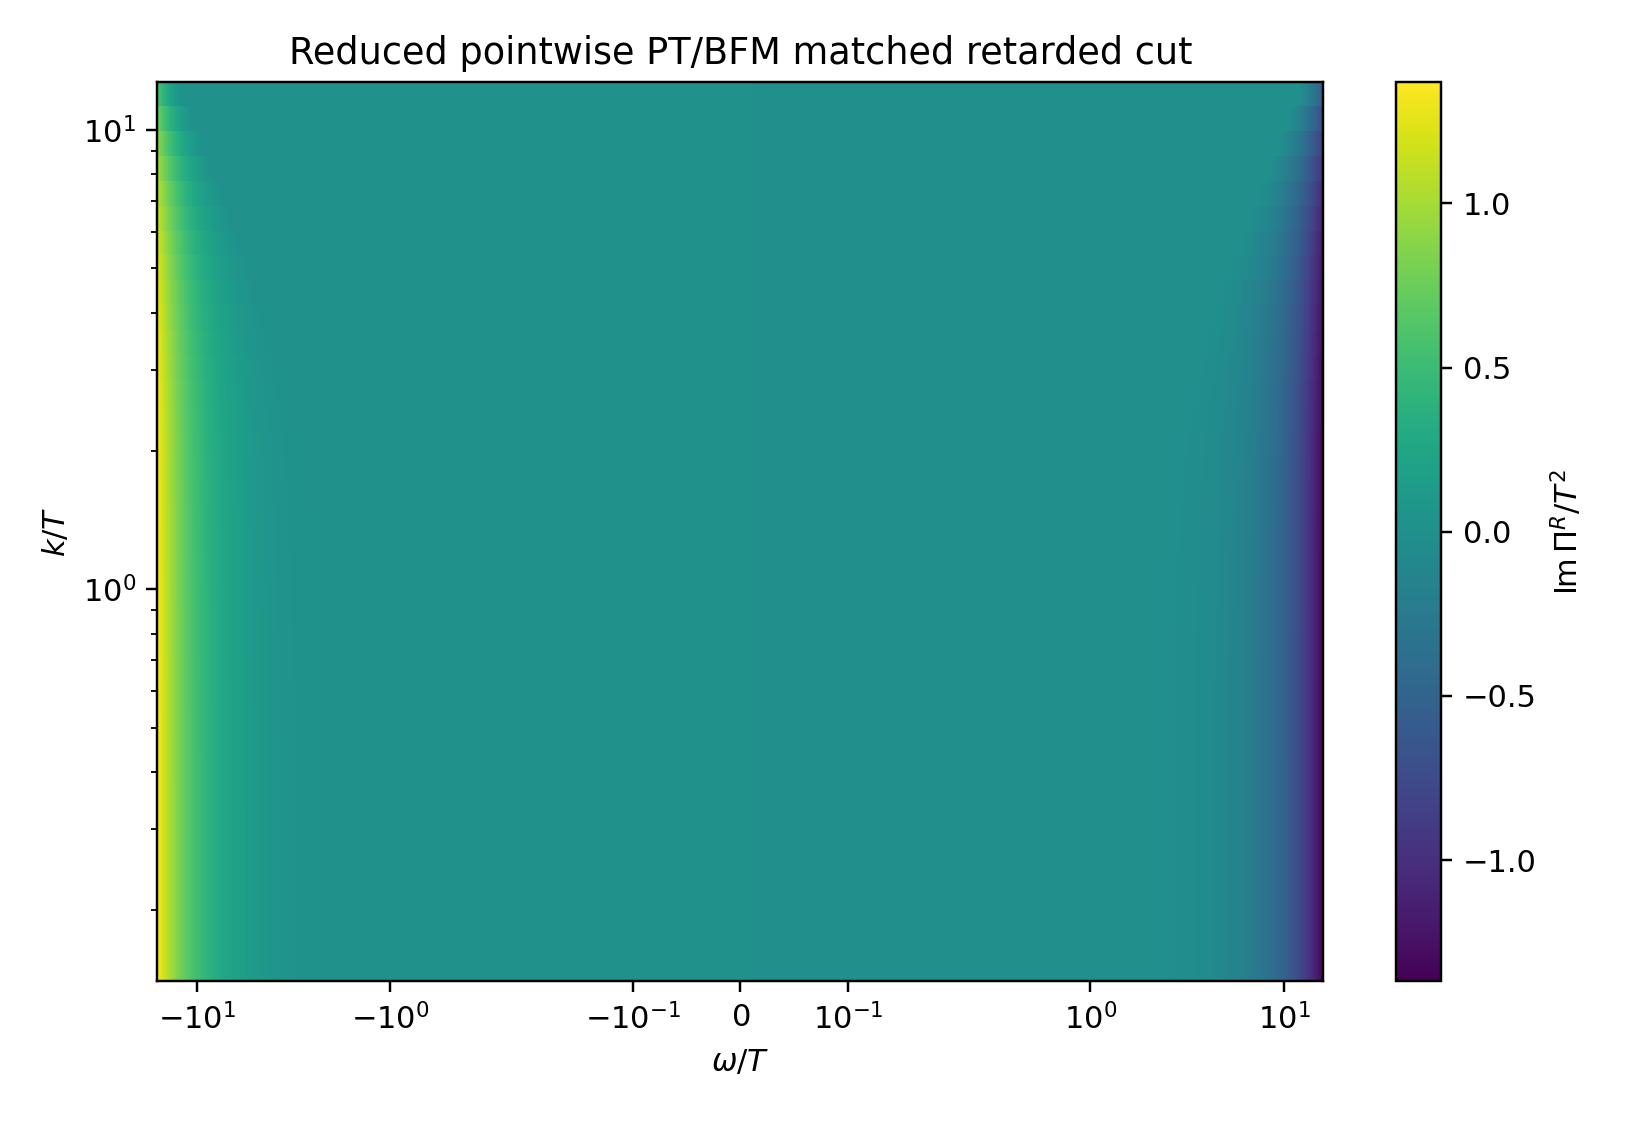
\includegraphics[width=0.92\textwidth,height=\textheight]{prehpc_pointwise_matching_v1_8.png}
\caption{Pointwise matched retarded cut.}
\end{figure}

\section{4. Longitudinal and transverse vertex
closure}\label{longitudinal-and-transverse-vertex-closure}

\subsection{4.1 Longitudinal background
vertices}\label{longitudinal-background-vertices}

For a dressed inverse propagator \(S^{-1}(P)\), the line-integral vertex

\[
\Gamma_L^\mu(P+Q,P)
=
\int_0^1ds\,
\frac{\partial S^{-1}(P+sQ)}{\partial P_\mu}
\]

satisfies

\[
Q_\mu\Gamma_L^\mu
=
S^{-1}(P+Q)-S^{-1}(P).
\]

This is the appropriate initial longitudinal background vertex. The
pre-HPC regression preserves the v1.7 background-Ward residual at
approximately machine precision.

\subsection{4.2 Declared ghost and matter-ghost
kernel}\label{declared-ghost-and-matter-ghost-kernel}

For the quantum Slavnov-Taylor initialization, the benchmark uses a
finite ghost dressing \(F(Q^2)\) and a common scalar matter-ghost kernel
\(h(P,Q)\):

\[
H=\overline H=h(P,Q)\mathbf1.
\]

The declared identity is

\[
Q_\mu\Gamma^\mu
=
F(Q^2)h(P,Q)
\left[
S^{-1}(P+Q)-S^{-1}(P)
\right].
\]

The maximum numerical residual over 600 random momentum samples is

\[
\boxed{1.71\times10^{-15}.}
\]

This is an exact result for the declared ansatz. It is \textbf{not} the
complete finite-temperature non-Abelian matter-ghost kernel. In a
general medium the vertex contains a much larger tensor basis, and the
matrix-valued quark-ghost scattering kernel must be solved or evolved.

\subsection{4.3 Finite transverse form
factors}\label{finite-transverse-form-factors}

Ward and Slavnov-Taylor identities do not determine transverse vertices.
The pre-HPC initialization therefore uses four explicitly transverse
fermionic tensors:

\[
T_1^\mu=Q^2\gamma^\mu-Q^\mu\slashed Q,
\]

\[
T_2^\mu=\left(Q^2P^\mu-P\cdot Q\,Q^\mu\right)\mathbf1,
\]

\[
T_3^\mu=\left(Q^2u^\mu-u\cdot Q\,Q^\mu\right)\mathbf1,
\]

\[
T_4^\mu=\sigma^{\mu\nu}Q_\nu.
\]

The form factors satisfy a finite separable Bethe-Salpeter equation,

\[
\boldsymbol\tau
=
\boldsymbol\tau_0
+
\mathbf K_T\boldsymbol\tau,
\]

so

\[
\boldsymbol\tau
=
(\mathbf1-\mathbf K_T)^{-1}\boldsymbol\tau_0.
\]

The gauge-kernel expansion parameter at the benchmark is

\[
\lambda_G=5.8525\times10^{-3}.
\]

The median form factors are

\[
\operatorname{median}(\tau_i)
=
(4.12,1.80,1.44,1.13)\times10^{-3}.
\]

The maximum transverse contraction residual is

\[
\boxed{1.57\times10^{-16}.}
\]

The median transverse-to-longitudinal vertex norm is

\[
9.22\times10^{-5},
\]

and the maximum in the sampled domain is

\[
3.66\times10^{-4}.
\]

\begin{figure}
\centering
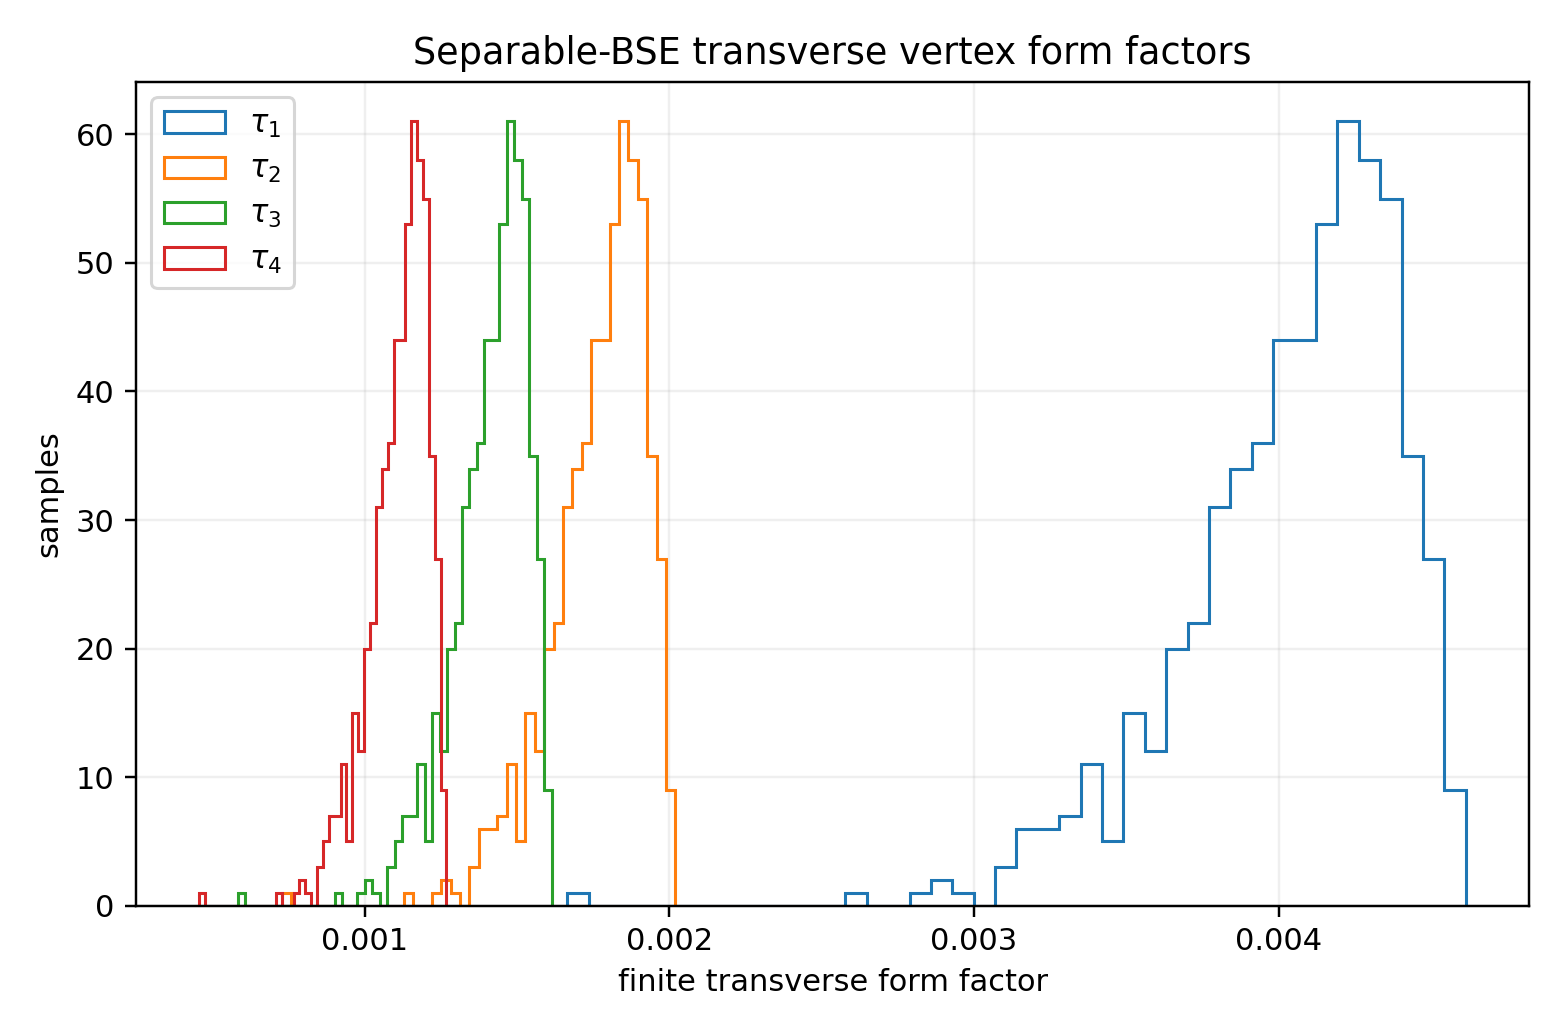
\includegraphics[width=0.88\textwidth,height=\textheight]{prehpc_transverse_vertices_v1_8.png}
\caption{Finite transverse form factors.}
\end{figure}

These small numbers should not be misread as a theorem that transverse
Standard-Model thermal vertices are always negligible. They are the
output of the declared weak-coupling separable initialization. The
production 3PI equations must evolve the transverse form factors and
report their effect on physical observables.

\section{\texorpdfstring{5. Gauge-singlet \(H^\dagger H\) control
correlator}{5. Gauge-singlet H\^{}\textbackslash dagger H control correlator}}\label{gauge-singlet-hdagger-h-control-correlator}

\subsection{5.1 Why the singlet control is
mandatory}\label{why-the-singlet-control-is-mandatory}

An elementary Higgs correlator can change away from the pole under a
gauge-parameter variation. A local BRST/gauge-invariant composite
operator provides a more physical spectral control.

Define

\[
\mathcal O_H=H^\dagger H.
\]

The earlier pole convolution supplied a useful baseline, but it did not
include a conserving ladder.

\subsection{5.2 Conserving separable
ladder}\label{conserving-separable-ladder}

Let \(\chi_0^R\) be the dressed two-particle bubble. The pre-HPC ladder
solves

\[
\Gamma_{\mathcal O}
=
1+K\chi_0^R\Gamma_{\mathcal O},
\]

and

\[
\chi_{\mathcal O}^R
=
\chi_0^R\Gamma_{\mathcal O}
=
\frac{\chi_0^R}{1-K\chi_0^R}.
\]

The scalar proxy uses

\[
K(k)=\frac{0.08}{1+(k/4T)^2}.
\]

The same declared kernel is interpreted as \(K=\delta\Sigma/\delta G\),
ensuring consistency between the self-energy proxy and response ladder.

The maximum algebraic BSE residual is

\[
\boxed{2.53\times10^{-16}.}
\]

The positive-frequency spectral density remains non-negative; its
minimum is

\[
4.91\times10^{-6}.
\]

The ladder changes the integrated spectral weight by between

\[
0.005\%\quad\text{and}\quad0.319\%,
\]

with maximum vertex enhancement

\[
1.00339.
\]

\begin{figure}
\centering
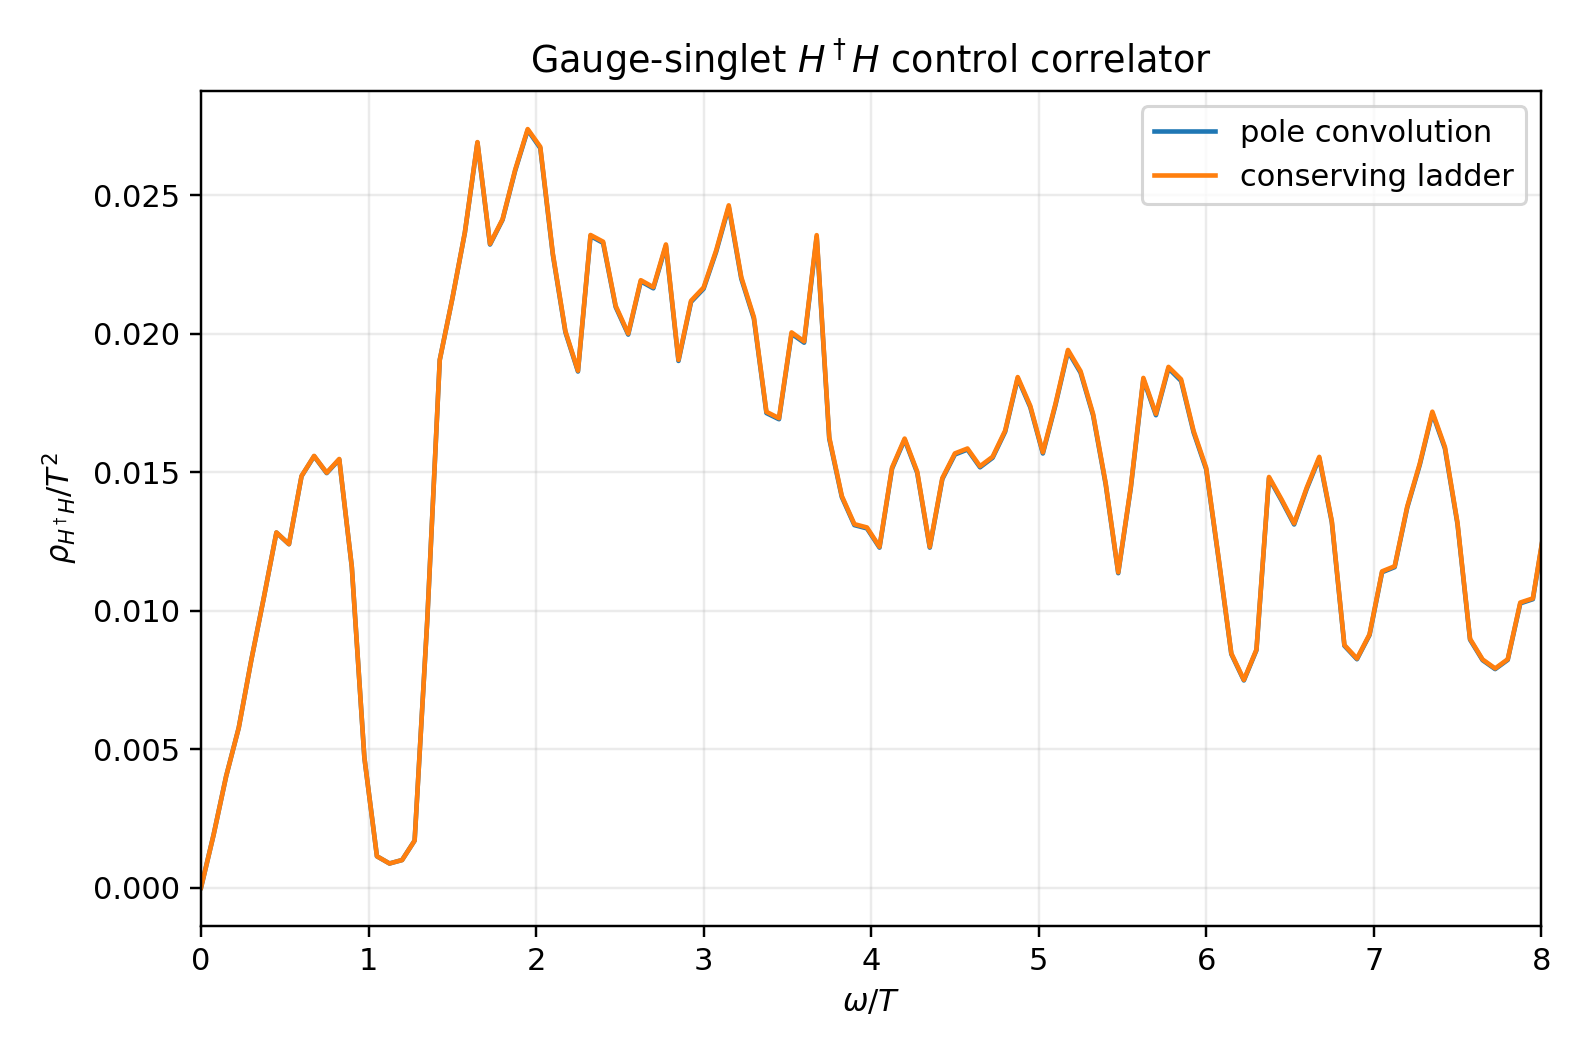
\includegraphics[width=0.88\textwidth,height=\textheight]{prehpc_singlet_bse_v1_8.png}
\caption{Gauge-singlet conserving ladder.}
\end{figure}

This is a conserving reduced control, not the final Standard-Model
composite-operator BSE. The production kernel must be generated from the
same 3PI truncation used for the propagators and vertices.

\section{6. What is now fixed for the HPC
run}\label{what-is-now-fixed-for-the-hpc-run}

\subsection{6.1 Dynamic variables}\label{dynamic-variables}

The solver specification includes two-point functions for

\[
H,Q,D,g,W,B,c_{SU(3)},c_{SU(2)},c_{U(1)},
\]

and three-point vertices for

\[
HqD,
\quad
AQQ,
\quad
ADD,
\quad
AHH,
\quad
AAA,
\quad
A\bar c c.
\]

The gauge-singlet \(H^\dagger H\) BSE is evolved as a control
observable.

\subsection{6.2 Truncation}\label{truncation}

The declared truncation is

\[
\boxed{
\text{three-loop 3PI in PT/BFM background Feynman gauge}
}
\]

with:

\begin{itemize}
\tightlist
\item
  line-integral/Ball-Chiu longitudinal initialization;
\item
  dynamic transverse three-point vertices;
\item
  explicit ghost dressing and matter-ghost kernels;
\item
  a quantum-gauge scan;
\item
  a conserving singlet ladder;
\item
  initial-surface counterterms;
\item
  hard-soft factorization-scale scans.
\end{itemize}

Again, the phrase ``PT/BFM-constrained'' is essential. Finite 3PI gauge
consistency is a numerical result to establish, not a property to
assume.

\subsection{6.3 Momentum and time
representation}\label{momentum-and-time-representation}

The pre-HPC resource model uses radial momentum and spherical harmonics:

\[
f(\mathbf p)=\sum_{\ell m}f_{\ell m}(p)Y_{\ell m}(\hat{\mathbf p}).
\]

This avoids storing a brute-force Cartesian three-momentum lattice while
retaining controlled anisotropy.

\begin{longtable}[]{@{}
  >{\raggedright\arraybackslash}p{(\columnwidth - 14\tabcolsep) * \real{0.0968}}
  >{\raggedleft\arraybackslash}p{(\columnwidth - 14\tabcolsep) * \real{0.1290}}
  >{\raggedleft\arraybackslash}p{(\columnwidth - 14\tabcolsep) * \real{0.1290}}
  >{\raggedleft\arraybackslash}p{(\columnwidth - 14\tabcolsep) * \real{0.1290}}
  >{\raggedleft\arraybackslash}p{(\columnwidth - 14\tabcolsep) * \real{0.1290}}
  >{\raggedleft\arraybackslash}p{(\columnwidth - 14\tabcolsep) * \real{0.1290}}
  >{\raggedleft\arraybackslash}p{(\columnwidth - 14\tabcolsep) * \real{0.1290}}
  >{\raggedleft\arraybackslash}p{(\columnwidth - 14\tabcolsep) * \real{0.1290}}@{}}
\toprule\noalign{}
\begin{minipage}[b]{\linewidth}\raggedright
Tier
\end{minipage} & \begin{minipage}[b]{\linewidth}\raggedleft
\(N_r\)
\end{minipage} & \begin{minipage}[b]{\linewidth}\raggedleft
\(\ell_{\max}\)
\end{minipage} & \begin{minipage}[b]{\linewidth}\raggedleft
momentum cells
\end{minipage} & \begin{minipage}[b]{\linewidth}\raggedleft
\(N_t\)
\end{minipage} & \begin{minipage}[b]{\linewidth}\raggedleft
memory window
\end{minipage} & \begin{minipage}[b]{\linewidth}\raggedleft
GPUs
\end{minipage} & \begin{minipage}[b]{\linewidth}\raggedleft
estimated aggregate memory
\end{minipage} \\
\midrule\noalign{}
\endhead
\bottomrule\noalign{}
\endlastfoot
Unit test & 32 & 1 & 128 & 512 & 64 & 1 & 0.11 GB \\
Pilot & 96 & 4 & 2,400 & 4,096 & 256 & 8 & 6.49 GB \\
Production angular-moment & 192 & 6 & 9,408 & 16,384 & 512 & 128 & 43.9
GB \\
\end{longtable}

The estimates include a factor-of-five workspace and checkpoint
overhead. They are architecture estimates, not vendor quotes.

\begin{figure}
\centering
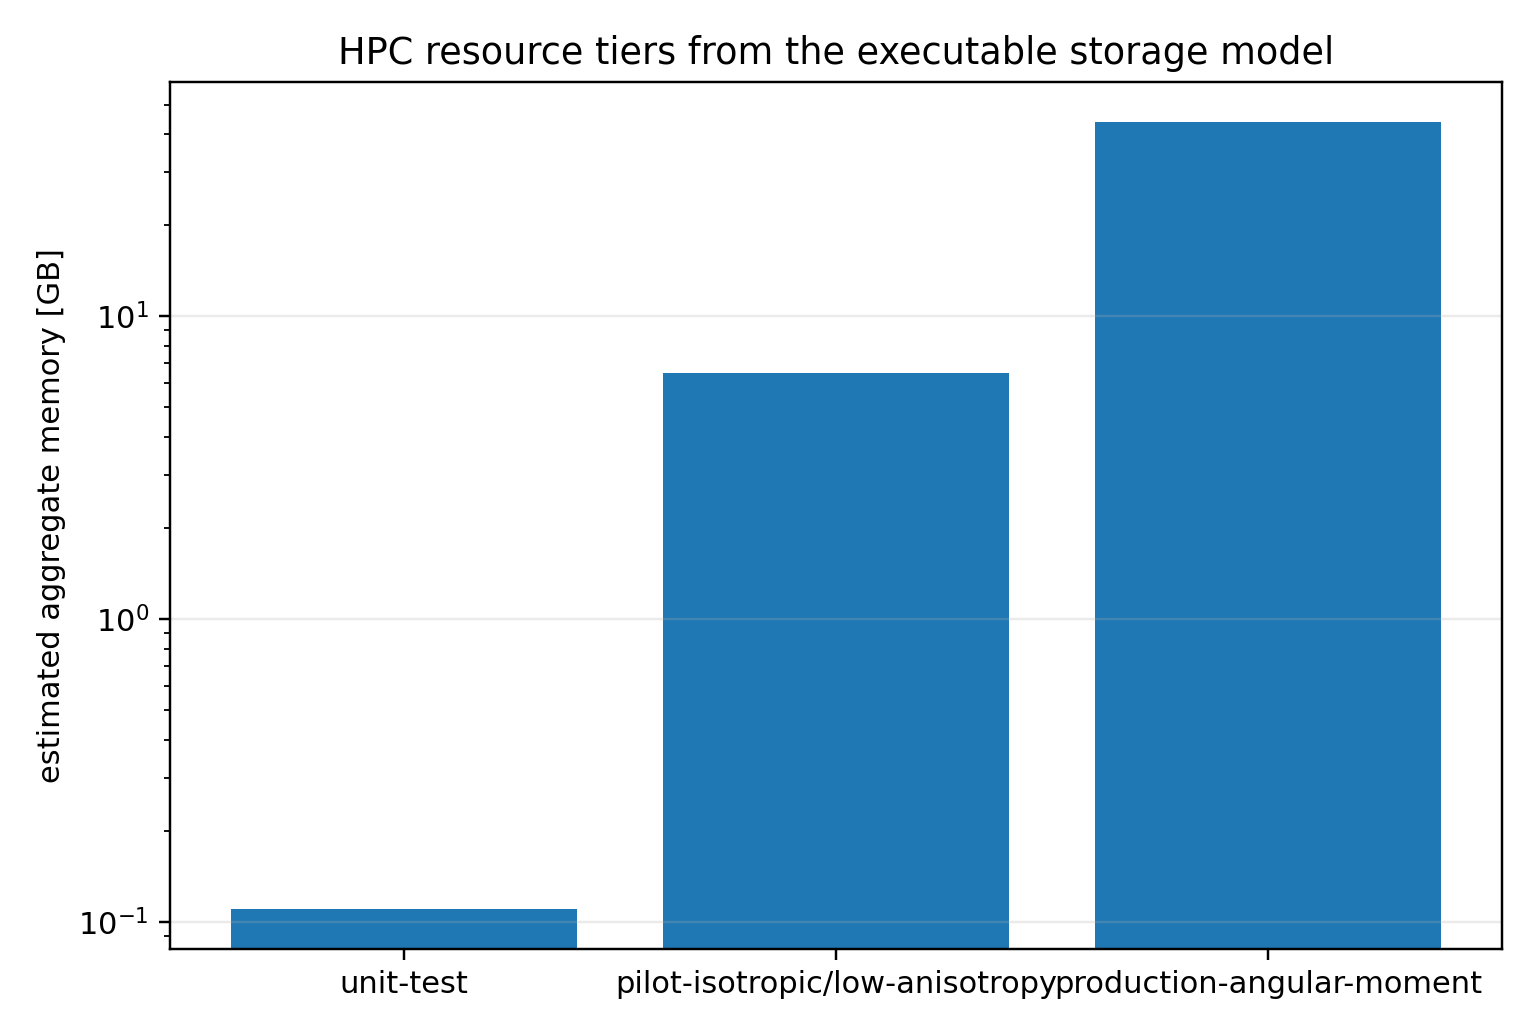
\includegraphics[width=0.82\textwidth,height=\textheight]{prehpc_resource_scaling_v1_8.png}
\caption{Resource scaling.}
\end{figure}

\subsection{6.4 Parallelization}\label{parallelization}

The recommended decomposition is:

\begin{itemize}
\tightlist
\item
  MPI over radial-angular momentum cells;
\item
  GPU tiles over memory time and vertex components;
\item
  deterministic global reductions for conservation diagnostics;
\item
  HDF5 checkpoints every 128 time steps;
\item
  float64 propagators and complex128 vertices in the pilot.
\end{itemize}

\section{7. Mandatory acceptance
gates}\label{mandatory-acceptance-gates}

A numerical run is rejected if any of the following fail:

\begin{longtable}[]{@{}lr@{}}
\toprule\noalign{}
Diagnostic & Pilot threshold \\
\midrule\noalign{}
\endhead
\bottomrule\noalign{}
\endlastfoot
On-shell width relative error & \(10^{-3}\) \\
Factorization-scale relative spread & \(10^{-5}\) \\
Background Ward residual & \(10^{-8}\) \\
Quantum STI residual & \(10^{-6}\) \\
Nielsen complex-pole spread & \(10^{-6}\) \\
KMS residual & \(10^{-7}\) \\
Equal-time commutator error & \(10^{-7}\) \\
Energy drift & \(10^{-6}\) \\
Gauge-charge drift & \(10^{-7}\) \\
Negative singlet spectral tolerance & \(10^{-10}\) \\
Singlet BSE residual & \(10^{-8}\) \\
Memory-window observable change & \(5\times10^{-3}\) \\
Gauge-parameter variation of physical observables & \(10^{-3}\) \\
\end{longtable}

These are launch thresholds, not theoretical identities. Production
tolerances should be tightened after the pilot establishes scaling.

\section{8. Automated preflight
result}\label{automated-preflight-result}

The packaged preflight performed the following checks:

\begin{longtable}[]{@{}ll@{}}
\toprule\noalign{}
Check & Result \\
\midrule\noalign{}
\endhead
\bottomrule\noalign{}
\endlastfoot
Factorization-scale cancellation & PASS \\
Exact on-shell anchor & PASS \\
Declared quantum STI & PASS \\
Singlet BSE equation & PASS \\
Singlet spectral positivity & PASS \\
KMS-noise positivity & PASS \\
\end{longtable}

The Python regression suite reports

\[
\boxed{4\ \text{tests passed}.}
\]

\section{9. What remains inside the HPC
calculation}\label{what-remains-inside-the-hpc-calculation}

The remaining work is no longer an ill-defined list of ``more exact
physics.'' It is the actual real-time simulation:

\begin{enumerate}
\def\labelenumi{\arabic{enumi}.}
\tightlist
\item
  evolve unequal-time propagators and three-point vertices
  self-consistently;
\item
  generate matrix-valued matter-ghost kernels rather than retaining the
  common-scalar initialization;
\item
  replace the reduced hard/LPM interpolation by the full differential
  real, virtual, HTL and LPM contributions;
\item
  evolve transverse vertices in the complete chosen tensor basis;
\item
  generate the \(H^\dagger H\) ladder kernel from the same
  time-dependent truncation;
\item
  demonstrate convergence with memory window, momentum resolution,
  angular moments and gauge parameter;
\item
  test whether physical observables remain stable even if individual
  off-shell elementary correlators vary.
\end{enumerate}

The most important output is not a pretty off-shell Higgs propagator. It
is the simultaneous satisfaction of:

\[
\boxed{
\text{physical anchors}
+
\text{Ward/ST closure}
+
\text{Nielsen stability}
+
\text{KMS}
+
\text{conservation}
+
\text{gauge-singlet agreement}.
}
\]

\section{10. Scientific status}\label{scientific-status}

The pre-HPC closure strengthens the project in three ways.

First, it removes a methodological ambiguity: bare-vertex 2PI and
unconstrained finite 3PI are not acceptable final methods.

Second, it provides a reproducible benchmark whose physical pole and
integrated rate are already controlled while every off-shell modelling
choice is labelled.

Third, it converts gauge consistency from rhetoric into a set of
numerical failure tests.

It does \textbf{not} by itself make the chronometric theory true. The
most publishable core remains the universal spectral-factorization
criterion, chronometric shear, and the QCD-transmitted
clock/equivalence-principle consistency relation. The real-time portal
work supports the viability of the cosmological realization; it is not
the conceptual theorem.

\section{11. Delivered files}\label{delivered-files}

The package includes:

\begin{itemize}
\tightlist
\item
  the technical note and PDF;
\item
  pointwise matching arrays;
\item
  finite transverse form factors and STI residuals;
\item
  singlet-ladder arrays;
\item
  the machine-readable HPC specification;
\item
  source code for loading kernels and running preflight tests;
\item
  unit tests;
\item
  resource estimates;
\item
  acceptance matrix;
\item
  figures and a complete archive.
\end{itemize}

\section{References}\label{references}

\begin{enumerate}
\def\labelenumi{\arabic{enumi}.}
\tightlist
\item
  J. Ghiglieri and M. Laine, \emph{Smooth interpolation between thermal
  Born and LPM rates}, arXiv:2110.07149.
\item
  G. Jackson and M. Laine, \emph{Efficient numerical integration of
  thermal interaction rates}, arXiv:2107.07132.
\item
  D. Bodeker and D. Schroder, \emph{Equilibration of right-handed
  electrons}, arXiv:1902.07220.
\item
  D. Binosi, \emph{Electroweak pinch technique to all orders},
  arXiv:hep-ph/0401182.
\item
  P. Gambino and P. A. Grassi, \emph{The Nielsen identities of the SM
  and the definition of mass}, arXiv:hep-ph/9907254.
\item
  J. Berges, \emph{n-Particle irreducible effective action techniques
  for gauge theories}, arXiv:hep-ph/0401172.
\item
  M. E. Carrington, A. R. Frey and B. A. Meggison, \emph{The gauge
  invariance of non-perturbative vertex prescriptions},
  arXiv:2606.27213.
\item
  D. M. van Egmond, \emph{Working towards a gauge-invariant description
  of the Higgs model}, arXiv:2310.06146.
\item
  M. E. Carrington, \emph{Transport coefficients and nPI effective
  actions}, arXiv:0912.3149.
\item
  J. M. Pawlowski et al., finite-temperature functional studies of
  non-Abelian vertices and Slavnov-Taylor constraints, including
  arXiv:1810.12938 and related work.
\end{enumerate}

\end{document}
